\documentclass[a4paper,14pt]{extarticle}

\newcommand{\stend}{\textbf{Wb-demo-kit v.2}}

% Путь до папки с общими шаблонами
\newcommand{\pathToCommonFolder}{/home/denilai/Documents/repos/latex/Common}

% Название работы в титуле
\newcommand{\workname}{Отчет по лабораторной работе № 5}
% Название дисциплины в титуле
\newcommand{\discipline}{Инструментальные средства разработки
	вычислительных систем}
% Название кафедры в титуле
\newcommand{\kafedra}{Кафедра вычислительной техники}
% Тема работы в титуле
\newcommand{\theme}{Работа с процессами}
% Должность преподавателя в титуле
\newcommand{\rang}{}

% ФИО студента в титуле
\newcommand{\studentfio}{К.~Ю.~Денисов}%\\Д.~Н.~Федосеев\\А.~М.~Сосунов}\\%К.~Ю.~Денисов\\%И.~А.~Кремнев
% ФИО преподавателя в титуле
\newcommand{\teacherfio}{И.~Р.~Сон}


\usepackage{tabularx}
\usepackage{lastpage}


\usepackage{booktabs}
\newcolumntype{b}{X}
\newcolumntype{s}{>{\hsize=.5\hsize}X}
\newcommand{\heading}[1]{\multicolumn{1}{|c|}{#1}}

% установка размера шрифта для всего документа
%\fontsize{20pt}{18pt}\selectfont
\usepackage{extsizes} % Возможность сделать 14-й шрифт

% Вставка заготовки преамбулы
% Этот шаблон документа разработан в 2014 году
% Данилом Фёдоровых (danil@fedorovykh.ru) 
% для использования в курсе 
% <<Документы и презентации в \LaTeX>>, записанном НИУ ВШЭ
% для Coursera.org: http://coursera.org/course/latex .
% Исходная версия шаблона --- 
% https://www.writelatex.com/coursera/latex/5.3

% В этом документе преамбула

% Для корректного использования русских символов в формулах
% пакеты hyperref и настройки, связанные с ним, стоит загуржать
% перед загрузкой пакета mathtext



% поддержка русских букв
% кодировка шрифта
%\usepackage[T2A]{fontenc} 
\usepackage{pscyr}

% использование ненумеровонного абзаца с добавлением его в содержаниеl

\newcommand{\anonsection}[1]{\section*{#1}\addcontentsline{toc}{section}{#1}}
\newcommand{\sectionunderl}[1]{\section*{\underline{#1}}}


% настройка окружения enumerate
\usepackage{enumitem}
\setlist{noitemsep}
\setlist[enumerate]{labelsep=*, leftmargin=1.5pc}

\usepackage{hyperref}

% сначала ставить \usepackage{extsizes} % Возможность сделать 14-й шрифт
% для корректной установки полей вставлять преамбулу следует в последнюю очередь (но перед дерективой замены \rmdefault)
\usepackage[top=20mm,bottom=25mm,left=35mm,right=20mm]{geometry} % Простой способ задавать поля

\hypersetup{				% Гиперссылки
	unicode=true,           % русские буквы в раздела PDF
	pdftitle={Заголовок},   % Заголовок
	pdfauthor={Автор},      % Автор
	pdfsubject={Тема},      % Тема
	pdfcreator={Создатель}, % Создатель
	pdfproducer={Производитель}, % Производитель
	pdfkeywords={keyword1} {key2} {key3}, % Ключевые слова
	colorlinks=true,       	% false: ссылки в рамках; true: цветные ссылки
	linkcolor=red,          % внутренние ссылки
	citecolor=black,        % на библиографию
	filecolor=magenta,      % на файлы
	urlcolor=blue           % на URL
}

%%% Работа с русским языком
\usepackage{cmap}					% поиск в PDF
\usepackage{mathtext} 				% русские буквы в формулах
\usepackage[T2A]{fontenc}			% кодировка
\usepackage[utf8]{inputenc}			% кодировка исходного текста
\usepackage[english,russian]{babel}	% локализация и переносы
\usepackage{indentfirst}
\frenchspacing

%для изменения названия списка иллюстраций
\usepackage{tocloft}


\renewcommand{\epsilon}{\ensuremath{\varepsilon}}
\renewcommand{\phi}{\ensuremath{\varphi}}
\renewcommand{\kappa}{\ensuremath{\varkappa}}
\renewcommand{\le}{\ensuremath{\leqslant}}
\renewcommand{\leq}{\ensuremath{\leqslant}}
\renewcommand{\ge}{\ensuremath{\geqslant}}
\renewcommand{\geq}{\ensuremath{\geqslant}}
\renewcommand{\emptyset}{\varnothing}

% Изменения параметров списка иллюстраций
\renewcommand{\cftfigfont}{Рисунок } % добавляем везде "Рисунок" перед номером
\addto\captionsrussian{\renewcommand\listfigurename{Список иллюстративного материала}}

\newcommand{\tm}{\texttrademark\ }
\newcommand{\reg}{\textregistered\ }


%%% Дополнительная работа с математикой
\usepackage{amsmath,amsfonts,amssymb,amsthm,mathtools} % AMS
\usepackage{icomma} % "Умная" запятая: $0,2$ --- число, $0, 2$ --- перечисление

%% Номера формул
%\mathtoolsset{showonlyrefs=true} % Показывать номера только у тех формул, на которые есть \eqref{} в тексте.
%\usepackage{leqno} % Нумереация формул слева

%% Свои команды
\DeclareMathOperator{\sgn}{\mathop{sgn}}

%% Перенос знаков в формулах (по Львовскому)
\newcommand*{\hm}[1]{#1\nobreak\discretionary{}
{\hbox{$\mathsurround=0pt #1$}}{}}


% отступ для первого абзаца главы или параграфа
%\usepackage{indentfirst}

%%% Работа с картинками
\usepackage{graphicx}  % Для вставки рисунков
\graphicspath{{images/}{screnshots/}}  % папки с картинками
\DeclareGraphicsExtensions{.pdf,.png,.jpg}
\setlength\fboxsep{3pt} % Отступ рамки \fbox{} от рисунка
\setlength\fboxrule{1pt} % Толщина линий рамки \fbox{}
\usepackage{wrapfig} % Обтекание рисунков текстом

%%% Работа с таблицами
\usepackage{array,tabularx,tabulary,booktabs} % Дополнительная работа с таблицами
\usepackage{longtable}  % Длинные таблицы
\usepackage{multirow} % Слияние строк в таблице

%%% Теоремы
\theoremstyle{plain} % Это стиль по умолчанию, его можно не переопределять.
\newtheorem{theorem}{Теорема}[section]
\newtheorem{proposition}[theorem]{Утверждение}

\theoremstyle{plain} % Это стиль по умолчанию, его можно не переопределять.
\newtheorem{work}{Практическая работа}[part]


 
 
\theoremstyle{definition} % "Определение"
\newtheorem{corollary}{Следствие}[theorem]
\newtheorem{problem}{Задача}[section]
 
\theoremstyle{remark} % "Примечание"
\newtheorem*{nonum}{Решение}



%%% Программирование
\usepackage{etoolbox} % логические операторы

%%% Страница

%	\usepackage{fancyhdr} % Колонтитулы
% 	\pagestyle{fancy}
%   \renewcommand{\headrulewidth}{0pt}  % Толщина линейки, отчеркивающей верхний колонтитул
% 	\lfoot{Нижний левый}
% 	\rfoot{Нижний правый}
% 	\rhead{Верхний правый}
% 	\chead{Верхний в центре}
% 	\lhead{Верхний левый}
%	\cfoot{Нижний в центре} % По умолчанию здесь номер страницы

\usepackage{setspace} % Интерлиньяж
\onehalfspacing % Интерлиньяж 1.5
%\doublespacing % Интерлиньяж 2
%\singlespacing % Интерлиньяж 1

\usepackage{lastpage} % Узнать, сколько всего страниц в документе.

\usepackage{soul} % Модификаторы начертания


\usepackage[usenames,dvipsnames,svgnames,table,rgb]{xcolor}


\usepackage{csquotes} % Еще инструменты для ссылок

%\usepackage[style=authoryear,maxcitenames=2,backend=biber,sorting=nty]{biblatex}

\usepackage{multicol} % Несколько колонок

\usepackage{tikz} % Работа с графикой
\usepackage{pgfplots}
\usepackage{pgfplotstable}

% модуль для вставки рыбы
\usepackage{blindtext}

\usepackage{listings}
\usepackage{color}


% для поворота отдельной страницы. Использовать окружение \landscape
\usepackage{pdflscape} 
\usepackage{rotating} 


\definecolor{mygreen}{rgb}{0,0.6,0}
\definecolor{mygray}{rgb}{0.5,0.5,0.5}
\definecolor{mymauve}{rgb}{0.58,0,0.82}


% пример импорта файла
%\lstinputlisting{/home/denilai/repomy/conf/distributions}

\lstset{
	language=Python,
	basicstyle=\footnotesize,        % the size of the fonts that are used for the code
	numbers=left,                    % where to put the line-numbers; possible values are (none, left, right)
	numbersep=5pt,                   % how far the line-numbers are from the code
	numberstyle=\tiny\color{mygray}, % the style that is used for the line-numbers
	stepnumber=2,                    % the step between two line-numbers. If it's 1, each line will be numbered
	% Tab - 2 пробела
	tabsize=2,    
	% Автоматический перенос строк
	breaklines=true,
	frame=single,
	breakatwhitespace=true,
	title=\lstname 
}





\setcounter{withouttheme}{0}
\setcounter{withoutsubmissiondate}{1}


%если нужна тема работы в отчете, то указать в скобках 0, иначе 1
%\setcounter{withouttheme}{0}
%если нужна дата представления отчета, то указать в скобках 0, иначе 1
%\setcounter{\withoutsubmissiondate}{0}

% установка полуторного интервала
% \usepackage{setspace}  
% \onehalfspacing

% использовать Times New Roman
\renewcommand{\rmdefault}{ftm}


\newcommand{\tb}{ThingsBoard~}

\begin{document}
	\thispagestyle{empty}
	% Вставка первого титульного листа
	% Есть две версии титульного листа - одиночный (titul) и групповой (titulAll)
	%\newcounter{withouttheme}

%\setcounter{withouttheme}{<n>} установить значение счетчика  withouttheme для определения, нужна ли тема
%    {0} - нужна
%    {1} - не нужна

%\setcounter{withoutsubmissiondate}{<n>} установить значение счетчика  withoutsubmissiondate для определения, нужна ли дата представления к защите
%     {0} - нужна
%     {1} - не нужена
\begin{center}
	\begin{figure}[h!]
		\begin{center}
		%\vspace{-10ex}
		
\includegraphics[width=0.17\linewidth]{\pathToCommonFolder/gerb}
		%\caption{}\label{pic:first}
		%	\vspace{5ex}
		\end{center}	
	\end{figure}
 	\small	МИНОБРНАУКИ РОССИИ \\
	Федеральное государственное бюджетное образовательное учреждение\\
						высшего образования\\
\normalsize					
\textbf{«МИРЭА – Российский технологический университет»\\
						РТУ МИРЭА}\\
						\noindent\rule{1\linewidth}{1pt}\\
       Институт информационных технологий\\ %\vspace{2ex}
					\kafedra\\
		\vspace{3ex}
			\large \textbf{\workname}  \\
		%\vspace{1ex}
						по дисциплине\\ «\discipline» \\
		\vspace{3ex}
		\ifnum \value{withouttheme}=0 {
			\textbf{Тема работы:}\\ <<\theme>>
		}
		\else {}
		\fi
\vspace{10ex}
\small
\begin{table}[h!]
\begin{tabular}{lp{0.6\linewidth}l}
	\textbf{Выполнил:} & студент группы ИВБО-02-19 & \\ 
	& & \studentfio \\%Д.~Н.~Федосеев\\%А.~М.~Сосунов\\%К.~Ю.~Денисов\\%И.~А.~Кремнев
	\textbf{Принял:} & \rang & \\
	& & \teacherfio \hfill\\
\end{tabular}
\end{table}
\end{center}
\ifnum \value{withoutsubmissiondate}=0 {
	\begin{flushleft}
		Работа представлена к защите <<\rule{3ex}{1pt}>>\rule{10ex}{1pt} 202\rule{1ex}{1pt} г.\hfill
	\end{flushleft}
\else {}
\fi

\normalsize
\begin{center}	
\vfill
Москва 2022
\end{center}

	\newpage
%	\tableofcontents
%	\newpage
	%\listoftables
	
\normalsize

\section*{Цель работы}
Цель лабораторной работы изучить программные средства
создания процессов, получить навыки управления и
синхронизации процессов.
\section*{Задание}
Написать программу в которой будет продемонстрировано создание и управление процессом-потомком.


\section*{Ход работы}
\subsection*{Создание процессов}
С целью демонстрации процесса создания процессов-потомков была написана программа на языке программирования C, исходный код которой приведен в листинге \ref{lst:fork}.
\begin{lstlisting}[language=C, caption={fork-demo.c}, label={lst:fork}]
	#include <unistd.h>
	#include <stdio.h>
	#include <stdlib.h>
	#include <sys/types.h>
	#include <sys/wait.h>
	
	int main(){
		pid_t t;
		int a;
		a=89;
		int status;
		printf("Before creating a descendant process a = %d\n",a);
		t=fork();
		if(t<0){
			perror("ERROR: Child process creation failed\n");
			return 1;
		}
		if(t==0){
			printf("In the child process a = %d\n",a);
			printf("Child PID = %d\n",getpid());
			printf("Parrent PID = %d\n",getppid());
			exit(1);
		}
		if (t>0)
		{
			a = 10;
			printf("a = 10\n");
			printf("In the parent process a = %d\n",a);
			printf("Parent PID =  %d\n",getpid());
			printf("Child PID =  %d\n",t);
			wait(&status);
			printf("wait() function argument =  0x%04x\n" , status);
		}
		return 0;
	}
\end{lstlisting}


В данной программе создается дочерний процесс, который представляет собой
точную копию своего процесса-предка.

Единственное различие
между ними заключается в том, что процесс-потомок в качестве
возвращаемого значения системного вызова \textit{fork() }получает 0, а
процесс-предок -идентификатор процесса-потомка. 

Кроме того,
процесс-потомок наследует и весь контекст программной среды,
включая дескрипторы файлов, каналы и т.д.

Ожидание завершения процесса-потомка родительским
процессом выполняется с помощью системного вызова wait()
int wait(int *status)

Аргумент системного вызова wait() представляет собой
указатель на целочисленную переменную status, которая после
завершения выполнения этого системного вызова будет
содержать в старшем байте код завершения процесса-потомка,
установленный последним в качестве системного вызова exit(), а
в младшем - индикатор причины завершения процесса-потомка.

Чтобы продемонстрировать, что дочерний процесс наследует все переменные родительского процесса, в начале функции main() была объявлена переменная a, значение которой изменялось по ходу программы. 

В данном случае дочерний процесс завершается с кодом 1, поэтому функция wait помещает в лидирующий байт аргумента значение 0x01.

Скомпилируем программу с помощью утилиты gcc с указанием исходного файла и выходного бинарного файла:
\texttt{gcc fork-demo.c -o fork-demo} (см. рисунок \ref{fig:demo}).

% TODO: \usepackage{graphicx} required
\begin{figure}[h!]
	\centering
	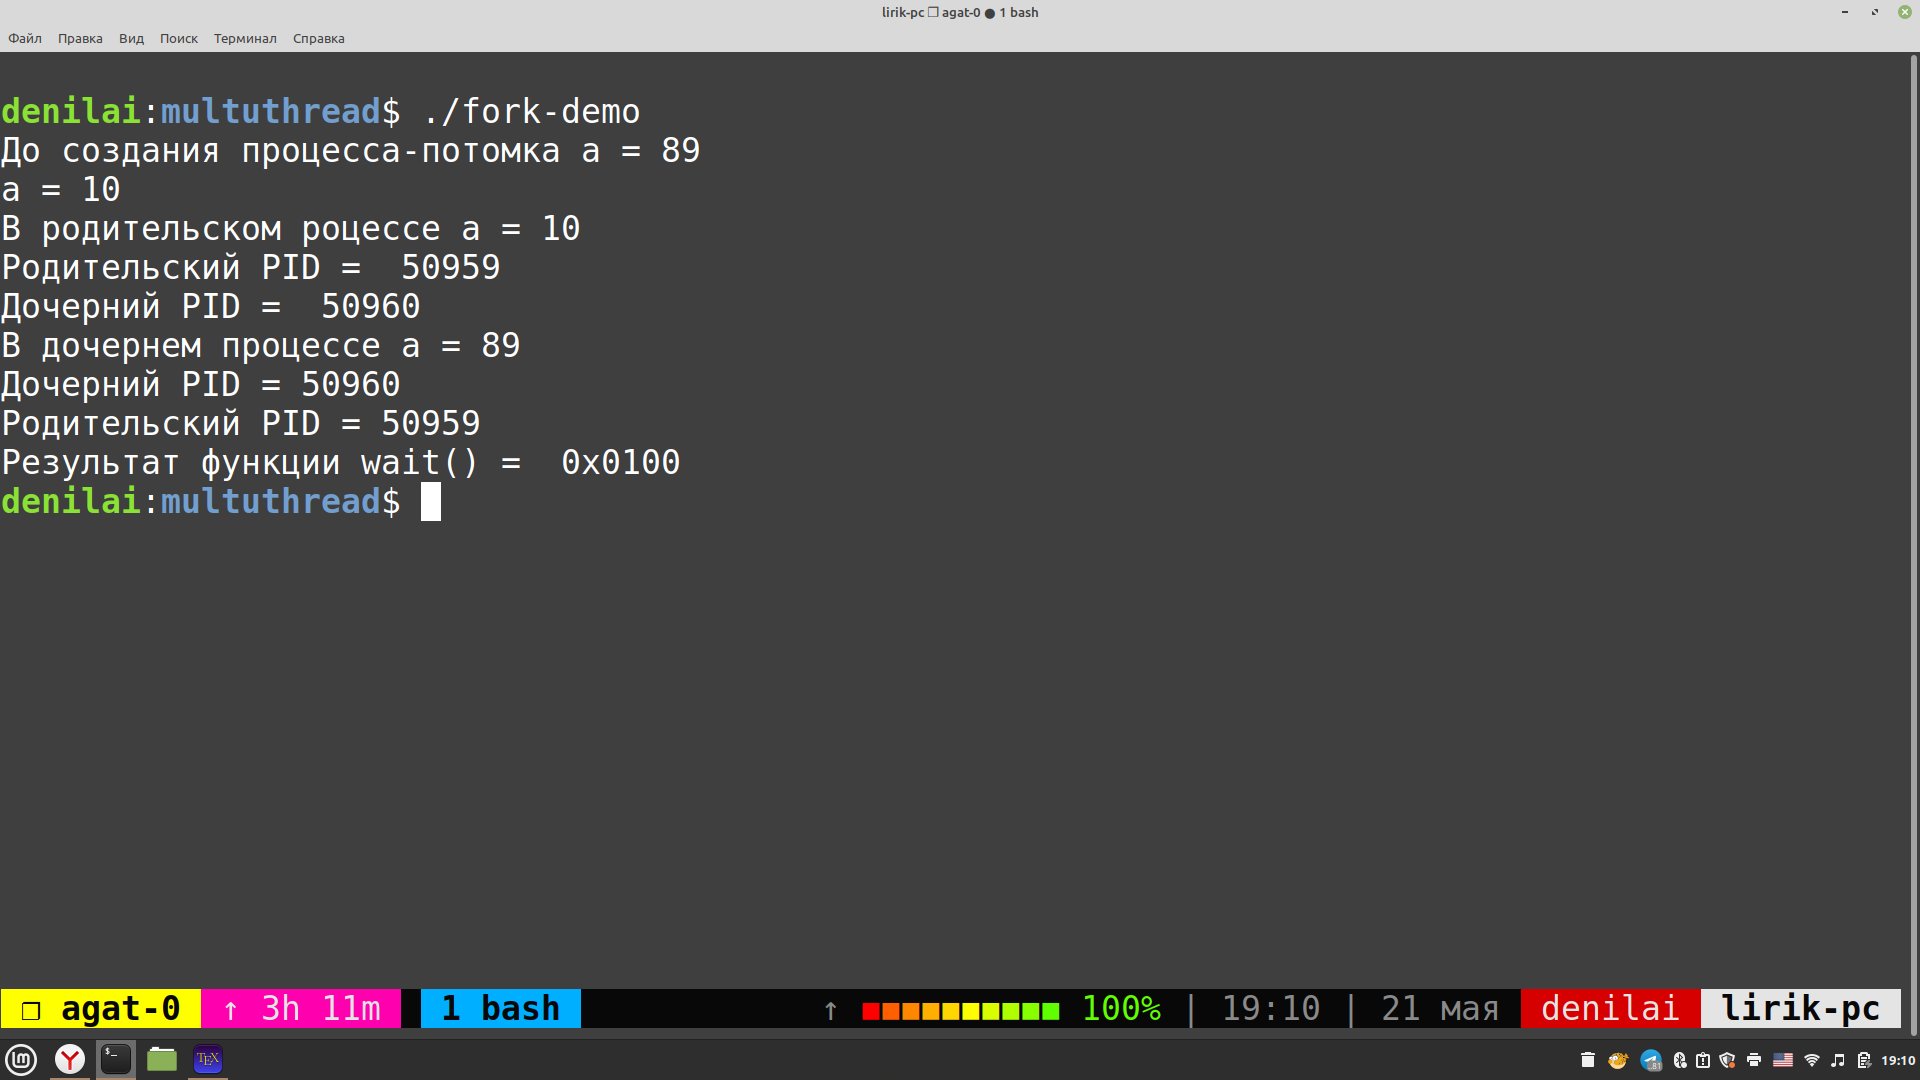
\includegraphics[width=0.9\linewidth]{images/5/demo}
	\caption{Запуск программы fork-demo}
	\label{fig:demo}
\end{figure}

\subsection*{Сигналы}
С целью демонстрации обработки сигналов была написана программа signals.c на языке программирования С, исходный код которой приведем в листинге \ref{lst:sig}.

\begin{lstlisting}[language=C, caption={signals.c}, label={lst:sig}]
	#include <stdlib.h>
	#include <stdio.h>
	#include <unistd.h>
	#include <sys/wait.h>
	#include <signal.h>
	
	void sigterm_handler(int sig){
		printf("\n=== handle SIGTERM ===\n\n");
	}
	
	int main (int argc, char* argv[]){
		int pid = fork();
		int chpid = getpid();
		if (pid == -1) {
			return 1;
		}
		if (pid == 0){
			void sigint_handler(int sig);
			char s[200];
			struct sigaction sa; 
			
			sa.sa_handler = sigint_handler;
			sa.sa_flags = 0;
			sigemptyset(&sa.sa_mask);
			if (sigaction(SIGTERM, &sa, NULL) == -1){
				perror("sigaction");
				exit(1);
			}
		
			while (1) {
				printf("We are in the child process with PID = %d\n", getpid());
				sleep(1);
			}
			return 0;
		}
		else {
			while (1){
				printf("Send SIGKILL signal to child process with PID = %d every 4 seconds\n", pid);
				sleep(3);
				kill(pid, SIGTERM);
			}
			wait(NULL);
		}
	}
	
\end{lstlisting}

В данной программе создается дочерний процесс, которому каждые 4 секунды отправляется сигнал SIGTERM. Дочерний процесс обрабатывает данный сигнал с помощью обработчика. Структура sigaction устанавливает обработчик и специальные флаги и маски. 

В результате при отправлении сигнала SIGTERM, дочерний процесс вызывает функцию sig\_handler().

Скомпилируем программу с помощью утилиты gcc с указанием исходного файла и выходного бинарного файла:
\texttt{gcc signals.c -o signals} (см. рисунок \ref{fig:demo1}).

% TODO: \usepackage{graphicx} required
\begin{figure}[h!]
	\centering
	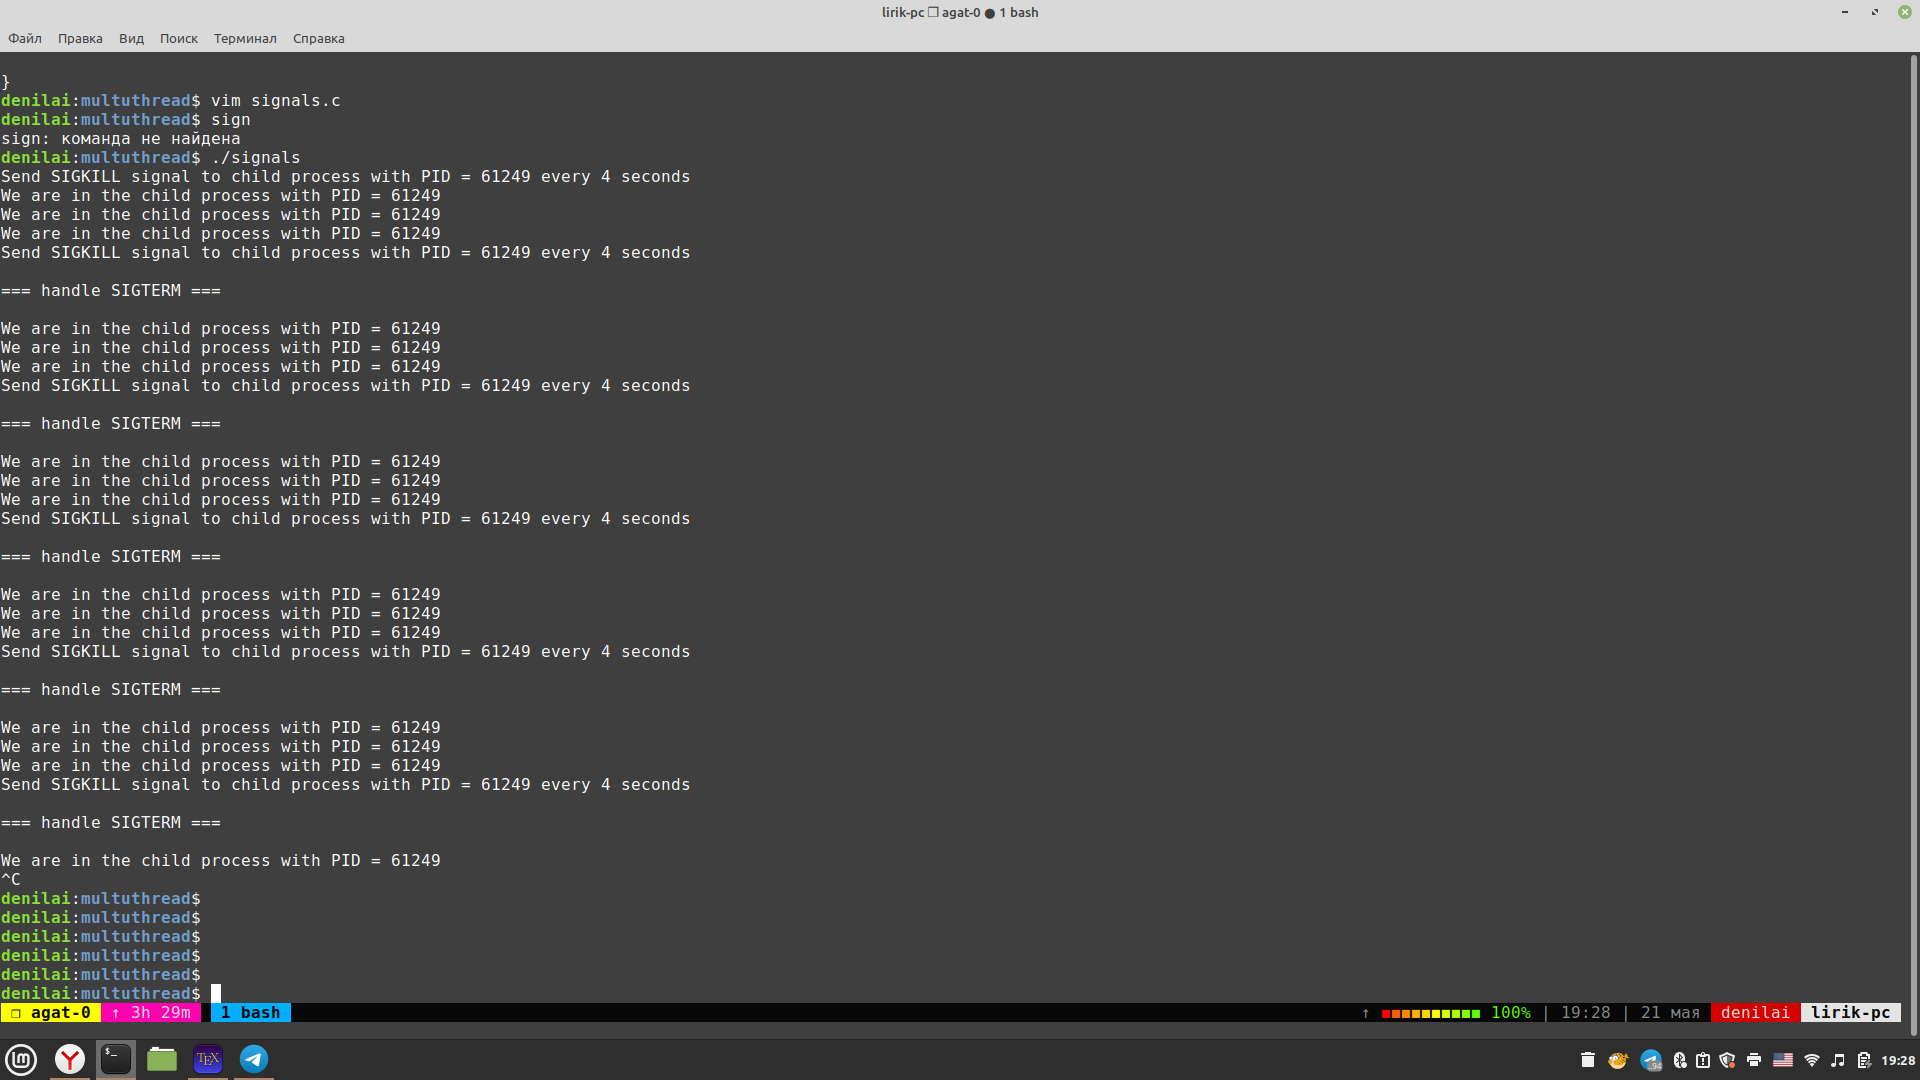
\includegraphics[width=0.9\linewidth]{images/5/demo1}
	\caption{Запуск программы signals}
	\label{fig:demo1}
\end{figure}



\newpage
\section*{Вывод}

В ходе настоящей лабораторной работы были созданы программы для демонстрации процесса создания процессов с помощью функции fork(), контроля изменения статуса дочернего процесса с помощью функции wait(), а также продемонстрирован способ обработки посылаемых сигналов.


\end{document}

